%%%%%%%%%%%%%%%%%%%%%%%%%%%%%%%%%%%%%%%%%%%%%%%%%%%%%%%%%%%%%%%%%%%%%%%%%%%%%%%%%%%%%%%%%%%%%%%%%%%%%%%%%%%%%%%%%%%%%%%%%%%%%%%%%%%
\chapter{DAE Compilation} \label{sec:dae-compilation} %%%%%%%%%%%%%%%%%%%%%%%%%%%%%%%%%%%%%%%%%%%%%%%%%%%%%%%%%%%%%%%%%%%%
%%%%%%%%%%%%%%%%%%%%%%%%%%%%%%%%%%%%%%%%%%%%%%%%%%%%%%%%%%%%%%%%%%%%%%%%%%%%%%%%%%%%%%%%%%%%%%%%%%%%%%%%%%%%%%%%%%%%%%%%%%%%%%%%%%%

Despite its potential, decoupling memory access from computation introduces substantial challenges for programmability. In scientific computing, this is less problematic because applications are typically built on libraries of standardized tensor algebra routines---such as BLAS~\cite{lawson1979blas}---that can be manually replaced with hand-optimized DAE implementations. In contrast, machine learning workloads are automatically compiled from high-level model descriptions, and their computational kernels are frequently fused. This makes manual DAE programming impractical and necessitates an automated approach.

Consequently, this chapter first introduces a programming model for expressing sparse machine learning operations on DAE architectures, using embedding operations and our TMU--CPU system as concrete examples. It then presents Ember, a generic compiler that lowers sparse machine learning operations to optimized DAE code. Ember is implemented in MLIR so that it can integrate with existing machine-learning compiler stacks, including PyTorch through torch-mlir and TensorFlow through its native MLIR compiler stack. The key idea behind Ember is to optimize DAE code at an intermediate level that exposes the access/execute split without losing the control-flow and data-flow information needed for global optimization. Finally, we show that Ember generates code whose performance matches that of hand-optimized implementations, unlocking the full potential of DAE architectures without imposing additional programmability burdens.

%%%%%%%%%%%%%%%%%%%%%%%%%%%%%%%%%%%%%%%%%%%%%%%%%%%%%%%%%%%%%%%%%%%%%%%%%%%%%%%%%%%%%%%%%%%%%%%%%%%%%%%%%%%%%%%%%%%%%%%%%%%%%%%%%%%
\section{DAE Programming Model} \label{sec:dae-programming-model} %%%%%%%%%%%%%%%%%%%%%%%%%%%%%%%%%%%%%%%%%%%%%%%%%%%%%%%%%%%%%%%%%%%%
%%%%%%%%%%%%%%%%%%%%%%%%%%%%%%%%%%%%%%%%%%%%%%%%%%%%%%%%%%%%%%%%%%%%%%%%%%%%%%%%%%%%%%%%%%%%%%%%%%%%%%%%%%%%%%%%%%%%%%%%%%%%%%%%%%%

This section outlines the programmability implications of separating memory access from computation into two distinct units for complex programs like embedding operations. We do so by formalizing our programming model for accelerating embedding operations and, more generally, sparse--dense tensor operations on DAE architectures.

\begin{figure}
\centering
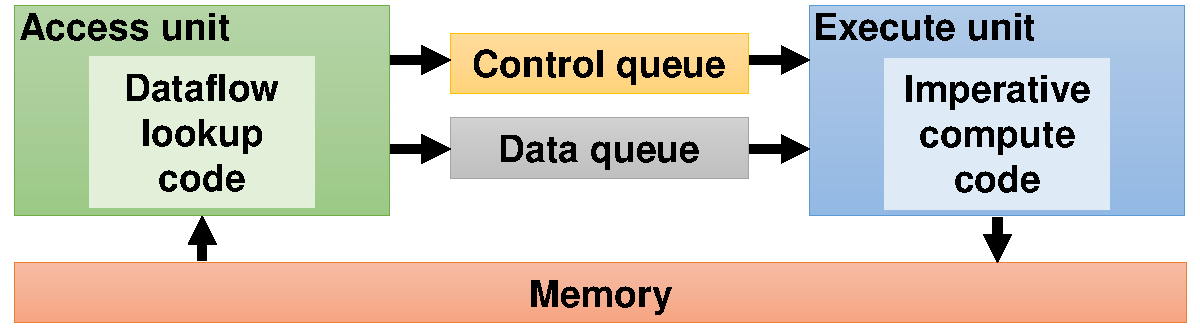
\includegraphics[width=.7\linewidth]{img_dae_abstraction.pdf}
\caption{DAE architectural abstraction.}
\label{fig:dae-abstraction}
\end{figure}

\Cref{fig:dae-abstraction} shows the logical DAE abstraction used by Ember for embedding operations on TMU--CPU systems and related DAE architectures~\cite{spzip2021isca,maple2022isca,planar2021acm}. Unlike the low-level TMU programming model introduced in \Cref{sec:tmu-architecture}, this abstraction does not expose hardware-specific details such as TUs, layers, lanes, merge modes, queue allocation, or outQ construction. Instead, it represents only the logical separation between lookup code, compute callbacks, and the queues that carry operands and control tokens between them. We call this low-level compiler abstraction the Decoupled Lookup--Compute (DLC) IR, which is the lowest-level IR of Ember, as explained in the next section.

The embedding operations targeted by Ember are sparse--dense tensor operations in which sparse metadata selects rows or blocks from dense tensors and the execute side performs elementwise reductions over the selected values~\cite{fusedmm2021ipdps}. For this class of programs, the lookup phase can be represented as a structured traversal hierarchy, and computation can be attached to the beginning, iteration, or end of each traversal loop~\cite{taco2017oopsla}. Unlike general sparse tensor algebra, these operations do not require sparse coordinate merging: the access unit traverses sparse metadata and performs indirect lookups, but it does not need to co-iterate multiple sparse fibers. Ember targets Einsum-style operators whose input and output tensors are distinct, so in-place updates are not part of the operator representation. Lookup operands are therefore read-only during a kernel, and output updates are handled by execute-side callbacks; consequently, the access unit does not depend on values produced by the execute unit during the same traversal.

Because of these properties, embedding operations can be expressed as a dataflow chain of access and compute blocks~\cite{sam2023asplos}. We can map lookup blocks to the access unit and compute blocks to the execute unit, and stream data and commands through logical queues. The DLC IR represents lookup blocks with streaming dataflow code, as it maps well to spatial architectures for memory-intensive workloads~\cite{sam2023asplos,spzip2021isca,fpga2022ccpe,topk2021dac,eigen2021fccm,fpga2021iwocl,cad2022tc}. Compute blocks, instead, are represented with imperative code, which can implement all the compute variants introduced above and other general-purpose computation. \Cref{fig:sls-lookup-code,fig:sls-compute-code} show the DLC IR for the EB function, which we discuss in the remainder of this section.

\begin{figure}
    \centering

    \begin{subfigure}{0.8\columnwidth}
        \centering
        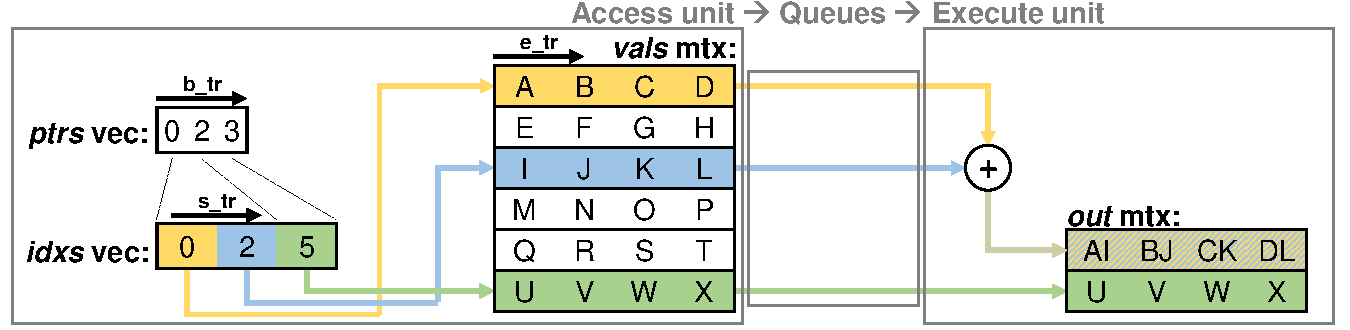
\includegraphics[width=\linewidth]{img_sls_example.pdf}
        \caption{Functional example of the EB function.}
        \label{fig:eb-functional-example}
    \end{subfigure}
    
    \begin{minipage}{\columnwidth}
    \begin{lstlisting}[xleftmargin=8pt]
void eb(idxs, ptrs, vals, out){
  for(int b = 0; b < num_batches; b++){ // Batch traversal (b_tr)
    for(int p = ptrs[b]; p < ptrs[b+1]; p++){ // Segment traversal (s_tr)
      idx = idxs[p]; // Load embedding index
      for(int e = 0; e < emb_len; e++){ // Embedding vec traversal (e_tr)
        val = vals[p,e]; // Load embedding element
        out[b,e] += val; }}}} // Reduce embedding elements
    \end{lstlisting}
    \vspace{-0.5em}
    \subcaption{Traditional imperative code, which also acts as input to Ember.}
    \label{fig:eb-imperative-code}
    \end{minipage}

    \begin{minipage}{\columnwidth}
    \begin{lstlisting}[xleftmargin=8pt]
 tr b_tr=loop_tr(0, num_batches, 1) // iterate thru batch
 str beg_ptr=b_tr.mem_str(ptrs, b_tr.ite) // load segment beg ptr
 str end_pos=b_tr.alu_str('+', b_tr.ite, 1) // compute next ptr pos
 str end_ptr=b_tr.mem_str(ptrs, end_pos) // load segment end ptr

 tr s_tr=loop_tr(beg_ptr, end_ptr, 1) // iterate thru segment
 str emb_idx=s_tr.mem_str(s_tr, idxs, s_tr.ite) // load emb idx
 str emb_beg=s_tr.alu_str(s_tr, '*', emb_idx, emb_len) // emb addr

 tr e_tr=loop_tr(0, emb_len, 1) // iterate thru emb vec
 str emb_pos=alu_str('+', emb_beg, e_tr.ite) // element addr
 str emb_val=mem_str(vals, emb_pos) // load emb element

 enq_op(b_tr.ite, e_tr, ite) // push batch position
 enq_op(e_tr.ite, e_tr, ite) // push emb el position
 enq_op(emb_val, e_tr, ite) // push emb el value
 callback(e_tr, ite) //trigger call on every emb iter
    \end{lstlisting}
    \vspace{-0.5em}
    \subcaption{DLC dataflow lookup code.}
    \label{fig:dlc-lookup-code}
    \end{minipage}
    
    \begin{subfigure}{\columnwidth}
        \centering
        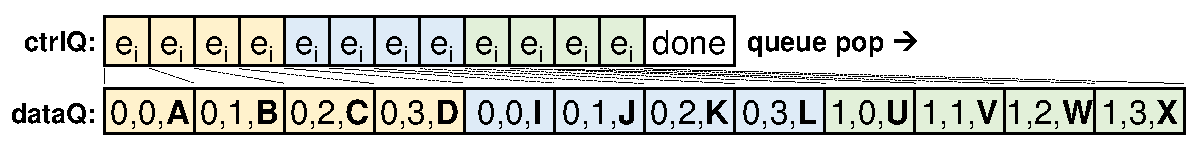
\includegraphics[width=0.81\columnwidth]{img_sls_queue.pdf}
        \caption{DLC queue content for the EB example.}
        \label{fig:dlc-queue-content}
    \end{subfigure}
    
    \begin{minipage}{\columnwidth}
    \begin{lstlisting}[xleftmargin=8pt]
while(ctrlQ.pop() == (*$e_i$*)){ // while some element
  b = dataQ.pop<1 x i32>(); // read embedding position
  e = dataQ.pop<1 x i32>(); // read element position
  v = dataQ.pop<1 x f32>(); // read element value
  fma(&out[b,e],v); // compute and store
    \end{lstlisting}
    \vspace{-0.5em}
    \subcaption{DLC imperative compute code.}
    \label{fig:dlc-compute-code}
    \end{minipage}
    %\vspace{-0.5em} % Adds vertical spacing between subfigures
    \caption[DLC representation of an EB operation.]{DLC representation of an EB operation. The functional example and imperative code define the source computation, the lookup code traverses batches, segments, and embedding elements with streams, the queues serialize callback tokens and operands, and the compute code dequeues those values to update the output. Overall, DLC separates embedding lookup from accumulation while preserving the callback order of the original loop nest.}
    \label{fig:dlc-eb-abstraction}
\end{figure}


The DLC lookup code loads embedding elements through memory streams. The IR uses index streams to maintain the iteration space for these memory streams, which are generated by traversal operators and can be transformed with integer ALU streams. Formally:
\begin{itemize}
    \item \textbf{\texttt{loop\_tr(lb,ub,stride)}}: creates a logical traversal over the iteration space \texttt{i=lb;i<ub;i+=stride}, where \texttt{lb} and \texttt{ub} are streams or immediate values and \texttt{stride} is an immediate value. The traversal handle exposes an \texttt{ite} stream containing the induction variable.
    \item \textbf{\texttt{mem\_str(base,idx)}}: loads into a stream the values of the \texttt{base} memory locations indexed by the \texttt{idx} stream.
    \item \textbf{\texttt{alu\_str(op,op1,op2)}}: computes an integer binary operation \texttt{op} $\in \{ +, -, \times, \div \}$ on operands \texttt{op1} and \texttt{op2}, which can either be streams or immediate values.
\end{itemize}
Concretely, we show these streams in the lookup code for the EB example in \Cref{fig:sls-lookup-code}. Lines 1--12 in \Cref{fig:sls-lookup-code} represent lines 5--9 in \Cref{fig:sls-imperative}, which are compiled by Ember.

Compute code consists of callbacks that the access unit triggers while traversing and loading tensor operands. In \Cref{fig:sls-imperative}, we can wrap the compute operation in line 10 into a callback that the access unit can trigger at each iteration of its parent loop. To trigger these callbacks, the access unit enqueues the corresponding token (the inner-loop iteration token ($e_i$)) in the control queue and its operands (result coordinates $b$ and $e$ and value $v$) in the data queue. Lines 14--17 in \Cref{fig:sls-lookup-code} and lines 2--4 in \Cref{fig:sls-compute-code} show how these tokens and data are enqueued and dequeued from the queues, and the exact queue content is shown in \Cref{fig:sls-queue}. \Cref{fig:opt-impact-idx} shows a more complex example with multiple callbacks. Formally, we can program the access unit to marshal control tokens and operands at three traversal locations---at each iteration, beginning, and end of a loop---through the following operations:
\begin{itemize}
    \item \textbf{\texttt{enq\_op(s\_id,tr\_id,event)}}: enqueues into the data queue (dataQ) the content of the \texttt{s\_id} stream every time a traversal \texttt{event} $\in \{ \texttt{beg}, \texttt{ite}, \texttt{end} \}$ occurs in \texttt{tr\_id}.
    \item \textbf{\texttt{callback(tr\_id,event)}}: enqueues into the control queue (ctrlQ) the corresponding control token every time a traversal \texttt{event} $\in \{ \texttt{beg}, \texttt{ite}, \texttt{end} \}$ occurs in \texttt{tr\_id}.
\end{itemize}
whereas the execute unit reads tokens and operands with:
\begin{itemize}
    \item \textbf{\texttt{deq()}}: dequeues a control token from the control queue.
    \item \textbf{\texttt{deq<ty>()}}: dequeues a value with \texttt{ty} type from dataQ.
\end{itemize}
We designed our DLC IR to express general embedding operations on various DAE architectures from the literature beyond the TMU, including:
\begin{itemize}
\item \textbf{SpZip}~\cite{spzip2021isca} integrates near-core specialized units in multicore processors to accelerate traversal and (de)compression operations in graph analytics. Similar to the TMU and other architectures for sparse tensor algebra~\cite{sam2023asplos}, SpZip's access unit can be programmed with a streaming language to traverse sparse data structures and send control tokens and data to the core, which can be programmed to process them with imperative languages. Hence, both the access and execute units can be abstracted with the DLC IR.
\item \textbf{MAPLE}~\cite{maple2022isca} offloads general indirect accesses to specialized units placed in the network-on-chip of a multicore processor. Access/compute units communicate through push/pull operations to/from queues, respectively. Unlike the TMU and SpZip, MAPLE access units are general-purpose cores. Hence, both access and execute code are imperative. The authors note that such code can be generated from sparse tensor compilers like TACO~\cite{taco2017oopsla}. Since SAM implements all hardware primitives of TACO and since the DLC IR can represent all SAM operations necessary for sparse-dense tensor operations, the DLC IR can abstract the MAPLE programming model.
\item \textbf{Planar}~\cite{planar2021acm} accelerates scientific workloads by offloading strided and irregular memory accesses from CPUs to tiny near-memory cores. Since Planar has a programming model similar to MAPLE, we can also abstract it with the DLC IR.
\end{itemize}
Ultimately, although separating embedding lookups from computation substantially improves performance and efficiency, it also introduces significant complexity into the DAE programming model, hindering the widespread adoption of DAE architectures. In the rest of this chapter, we demonstrate how the Ember compiler addresses this challenge by automatically targeting the DLC IR from standard imperative code and compiling down to DAE hardware code.

%%%%%%%%%%%%%%%%%%%%%%%%%%%%%%%%%%%%%%%%%%%%%%%%%%%%%%%%%%%%%%%%%%%%%%%%%%%%%%%%%%%%%%%%%%%%%%%%%%%%%%%%%%%%%%%%%%%%%%%%%%%%%%%%%%%
\section{The Ember Compiler} \label{sec:ember-compiler}
%%%%%%%%%%%%%%%%%%%%%%%%%%%%%%%%%%%%%%%%%%%%%%%%%%%%%%%%%%%%%%%%%%%%%%%%%%%%%%%%%%%%%%%%%%%%%%%%%%%%%%%%%%%%%%%%%%%%%%%%%%%%%%%%%%%

This section introduces Ember, a compiler we designed to automatically lower structured sparse machine learning operations to DAE architectures, enabling their full performance potential without additional programmability burden.

%%%%%%%%%%%%%%%%%%%%%%%%%%%%%%%%%%%%%%%%%%%%%%%%%%%%%%%%%%%%%%%%%%%%%%%%%%%%%%%%%%%%%%%%%%%%%%%%%%%%%%%%%%%%%%%%%%%%%%%%%%%%%%%%%%%
\subsection{Ember Overview} %%%%%%%%%%%%%%%%%%%%%%%%%%%%%%%%%%%%%%%%%%%%%%%%%%%%%%%%%%%%%%%%%%%%%%%%%%%%%%%%%%%%%%%%%%%%%%%%%%%%%%%%%%
%%%%%%%%%%%%%%%%%%%%%%%%%%%%%%%%%%%%%%%%%%%%%%%%%%%%%%%%%%%%%%%%%%%%%%%%%%%%%%%%%%%%%%%%%%%%%%%%%%%%%%%%%%%%%%%%%%%%%%%%%%%%%%%%%%%

\begin{figure}
    \centering
    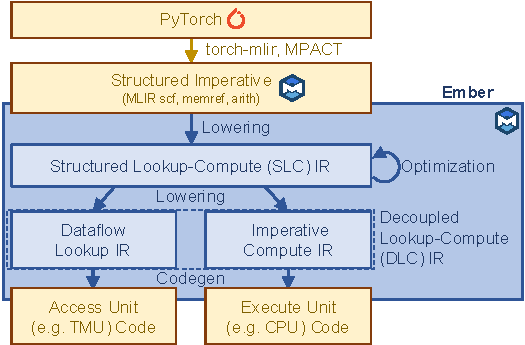
\includegraphics[width=0.7\columnwidth]{img_ember_overview_no_labels.pdf}
    \caption[Overview of the Ember compiler.]{Overview of Ember. \hlc[yellow!20]{Yellow} represents compiler inputs and outputs, and \hlc[blue!20]{blue} represents new contributions. Ember compiles a structured imperative IR into fully decoupled and optimized DAE code.}
    \label{fig:ember-overview}
\end{figure}

\Cref{fig:ember-overview} shows our MLIR~\cite{mlir2021cgo} implementation of Ember. Overall, Ember compiles structured representations of sparse machine learning operations into optimized DLC code, which is then used for DAE code generation. The Structured Control Flow (SCF) Dialect is perhaps the most popular structured IR in MLIR, and resembles the imperative code in \Cref{fig:sls-imperative}. Ember operates on structured MLIR, which enables integration with existing machine-learning compiler stacks. For example, PyTorch programs can enter Ember through torch-mlir~\cite{torchmlir2026github}, while TensorFlow programs can enter through TensorFlow's native MLIR compiler stack. Ember can also generate SCF from general tensor algebra expressions with tools like MPACT~\cite{mpact2021google}.

The compiler pipeline uses four levels of representation. SCF is the structured-loop input. Structured Lookup-Compute (SLC) is the optimization IR: it marks access streams and compute callbacks while preserving structured control flow and SSA-style data flow. DLC is the low-level DAE IR: it makes control and data queues explicit after global optimizations have been selected. Finally, target-specific dialects such as \texttt{tmu} and \texttt{llvm} generate code for the access and execute units.

To generate optimized DAE code from SCF, Ember needs to decouple memory accesses from computation and generate optimized code for the access unit and execute unit. However, the main challenge of this process is that DAE code cannot be optimized either in the DLC IR or in SCF alone. Global optimizations across access and execute code need the control flow and data flow of the entire input program, which are already lost and decoupled in the DLC IR. For instance, it would be impractical to identify what stream generates the \texttt{v} value in the DLC IR in \Cref{fig:opt-impact-idx}, which is an essential analysis for several optimizations discussed in \Cref{sec:ember-global-optimizations}. Instead, while SCF has knowledge of both control flow and data flow, it does not differentiate between access and execute code, nor does it identify how data is (de)serialized between them. Therefore, global optimizations would need to be integrated into the code separation and/or generation logic, which is impractical for a large set of complex optimizations, such as those in \Cref{sec:ember-global-optimizations}, that should be executed iteratively~\cite{mlir2021cgo}.

For this reason, we designed the Structured Lookup-Compute (SLC) IR (\Cref{sec:the-slc-ir}). The SLC IR is a natural extension of the SCF IR for DAE code. The key feature of the SLC IR is to represent DAE code while preserving the control flow and data flow of the input program, enabling iterative DAE optimizations across access and execute code. In this way, Ember decides what SCF operations to map to the access and execute units and generates the SLC IR (\Cref{sec:lowering-scf-to-slc}). Then, it performs global optimizations (\Cref{sec:ember-global-optimizations}) on the SLC IR and lowers it to the DLC IR for separate optimizations of access and execute code (\Cref{sec:lowering-slc-to-dlc}). Access and execute code are then lowered to target-specific IRs such as the \texttt{tmu} and \texttt{llvm} dialects, which are then used for code generation (\Cref{sec:code-generation}). Each step is presented in the following sections.

%%%%%%%%%%%%%%%%%%%%%%%%%%%%%%%%%%%%%%%%%%%%%%%%%%%%%%%%%%%%%%%%%%%%%%%%%%%%%%%%%%%%%%%%%%%%%%%%%%%%%%%%%%%%%%%%%%%%%%%%%%%%%%%%%%%
\subsection{SCF Decoupling and Lowering} \label{sec:scf-decoupling-and-lowering} %%%%%%%%%%%%%%%%%%%%%%%%%%%%%%%%%%%%%%%%%%%%%%%%%%%%%%%%%%%%%%%%%%%%%%
%%%%%%%%%%%%%%%%%%%%%%%%%%%%%%%%%%%%%%%%%%%%%%%%%%%%%%%%%%%%%%%%%%%%%%%%%%%%%%%%%%%%%%%%%%%%%%%%%%%%%%%%%%%%%%%%%%%%%%%%%%%%%%%%%%%

\begin{figure}
  \normalsize
\[
\begin{array}{rl|@{\hspace{1.5\arraycolsep}}rl}
\textit{Any CPU Statement} & STMT &
\textit{Memory Reference} & mref \\
\textit{CPU variable} & var &
\textit{Stream Variable} & s \\
\textit{Unsigned Integer} & \text{uint} \\
\end{array}
\]
\[
\begin{array}{rlrl}
  \textit{For-Loop} & FOR & \bnfdef & \text{for } (HEAD) \text{ \{ } SDEC^* ~ BODY \text{ \} }\\
  \textit{For Header} & HEAD & \bnfdef & s = r \text{ to } r \text{ step } \text{uint} \\
  \textit{Stream Declaration} & SDEC  & \bnfdef & s = se \\
  \textit{Loop Body} & BODY & \bnfdef & CALL ~\bnfalt~ CALL? ~~ FOR ~~ CALL? \\
  \textit{Callback} & CALL & \bnfdef & \text{callback()} \text{ \{ } TVAL^*~ STMT^+ \text{ \}} \\
  \textit{Value Conversion} & TVAL & \bnfdef & var = \text{to\_val}(s) \\
  \textit{Loop Range} & r & \bnfdef &  s ~\bnfalt~ var ~\bnfalt~ \text{uint}  \\
  \textit{Stream Expression} & se & \bnfdef & ls~\bnfalt~as~\bnfalt~cs~\bnfalt~bs \\
  \textit{Load Stream} & ls  & \bnfdef & \text{load\_str} (mref[indices^*], uint) \\
  \textit{Indices} & indices & \bnfdef & s~\bnfalt~var~\bnfalt~ \text{uint} \\
  \textit{ALU Stream} & as & \bnfdef & \text{alu\_str} (sop, s_1, s_2) \\
  \textit{Stream Ops} & sop  & \bnfdef & +~\bnfalt~-~\bnfalt~*~\bnfalt~ 
/~\bnfalt~\%~\bnfalt~ \ldots  \\
\end{array}
\]
  \caption[SLC IR grammar.]{Grammar of Ember's Structured Lookup--Compute (SLC) IR. The SLC IR represents structured loops, stream declarations, callbacks, and stream-to-value conversions in a single structured representation. In this way, SLC preserves the control flow and data flow needed for global DAE optimizations before the program is serialized into explicit DLC queues.}
  \label{fig:ember-slc-ir-grammar}
\end{figure}


This section introduces the SLC IR and explains how Ember lowers SCF code to it and lowers it to DLC code. This lowering has three responsibilities: identifying loop traversals that can run on the access unit, preserving computation that must remain on the execute unit as callbacks, and recording stream-to-value uses so later optimizations can reason across the access/execute boundary.

%%%%%%%%%%%%%%%%%%%%%%%%%%%%%%%%%%%%%%%%%%%%%%%%%%%%%%%%%%%%%%%%%%%%%%%%%%%%%%%%%%%%%%%%%%%%%%%%%%%%%%%%%%%%%%%%%%%%%%%%%%%%%%%%%%%
\subsubsection{The SLC IR} \label{sec:the-slc-ir} %%%%%%%%%%%%%%%%%%%%%%%%%%%%%%%%%%%%%%%%%%%%%%%%%%%%%%%%%%%%%%%%%%%%%%%%%%%%%%%%%%%%%%%%
%%%%%%%%%%%%%%%%%%%%%%%%%%%%%%%%%%%%%%%%%%%%%%%%%%%%%%%%%%%%%%%%%%%%%%%%%%%%%%%%%%%%%%%%%%%%%%%%%%%%%%%%%%%%%%%%%%%%%%%%%%%%%%%%%%%

\Cref{fig:slc-ir} shows the SLC grammar, and \Cref{fig:lowering-slc} shows the SLC IR of the EB function example. The main goal of the SLC IR is to abstract the queue (de)serialization logic in the DLC IR, enabling global DAE optimizations.

Similar to the DLC IR, the SLC IR defines access code (i.e. memory access and index arithmetic) through streams and compute code through callbacks. However, unlike the DLC IR, the SLC IR places these streams and callbacks within structured SLC imperative for-loops.

In this way, the value of the streams can be directly accessed from the callbacks through stream-to-value conversion operations, preserving the data flow of the input code. Semantically, an SLC stream produces one logical value per iteration of its defining loop. A callback observes stream values only through \texttt{to\_val} operations, which materialize the value associated with the callback event. The lexical position of callbacks in the loop body defines the callback order, and lowering to DLC preserves that order when emitting control tokens and operands into queues.

The SLC IR allows Ember to simultaneously optimize lookup and compute code through global analyses and transformations, including dominance analysis, vectorization, and code motion across different compute regions as well as across access and execute code. We later describe these analyses and optimizations that the SLC IR enables in more detail in \Cref{sec:ember-global-optimizations}.

%%%%%%%%%%%%%%%%%%%%%%%%%%%%%%%%%%%%%%%%%%%%%%%%%%%%%%%%%%%%%%%%%%%%%%%%%%%%%%%%%%%%%%%%%%%%%%%%%%%%%%%%%%%%%%%%%%%%%%%%%%%%%%%%%%%
\subsubsection{Lowering the SCF IR to the SLC IR} \label{sec:lowering-scf-to-slc} %%%%%%%%%%%%%%%%%%%%%%%%%%%%%%%%%%%%%%%%%%%%%%%%%%%%%%%%%%%
%%%%%%%%%%%%%%%%%%%%%%%%%%%%%%%%%%%%%%%%%%%%%%%%%%%%%%%%%%%%%%%%%%%%%%%%%%%%%%%%%%%%%%%%%%%%%%%%%%%%%%%%%%%%%%%%%%%%%%%%%%%%%%%%%%%

\Cref{fig:lowering} shows a lowering example from SCF to SLC. To generate the SLC IR, Ember recursively traverses the loop hierarchy of the SCF code looking for loops to offload to the access unit. We define an \emph{offloading candidate} as a loop that (1)~has iteration bounds that are either static or computed by another offloading candidate and (2)~loads from at least one read-only memory location that has not been read from a parent loop. Condition (1) is necessary because access units cannot generally read data from the execute units. Condition (2) excludes workspace loops~\cite{workspaces2019cgo,spworkspaces2024pldi} (i.e., loops that work only on partial results). As partial results are likely cached, workspace loops do not benefit from memory acceleration. All loops in \Cref{fig:lowering-scf} are offloading candidates. For a more complex example, only the first two loops from the MP pseudocode in \Cref{sec:characterization-and-implications} are offloading candidates. The last two lines (loops) in MP are workspace loops, as they just multiply and accumulate the temporary vector with the vertex vector, which has already been read.

The legality of this decoupling transformation follows from Ember's Einsum-style operator representation. Input tensors and the output tensor are distinct: input tensors are read-only, the output tensor is write-only, and the representation does not allow tensor overlap or in-place updates. As a result, moving input loads and index arithmetic to the access unit cannot introduce read-write conflicts or aliasing with output updates. Ember therefore offloads only operations whose operands are constants, loop induction variables, input-tensor loads, or values produced by other access-unit streams. Operations that write the output tensor, update partial results, or depend on execute-side values remain in callbacks. In this way, reductions and output stores stay on the execute unit, while read-only traversal and index computation move to the access unit.

\begin{figure}
    \noindent
    \begin{subfigure}[]{1\columnwidth}
        \begin{subfigure}[t]{0.47\columnwidth} %47
            \begin{lstlisting}[xleftmargin=1.5em]
void eb(idxs: mref<? x idx>,
         ptrs: mref<? x idx>,
         vals: mref<? x f32>,
         out: mref<? x ? x f32>){
 (*\hlloop{for(idx b=0; b<n\_batches; b++)}*){
  (*\hlmem{idx beg=ptrs[b]}*);
  (*\hlmem{idx end=ptrs[b+1]}*);
  (*\hlloop{for(idx p=beg; p<end; p++)}*){
   (*\hlmem{idx i=idxs[ptr]}*);
   (*\hlloop{for(idx e=0; e<emb\_len; e++)}*){
    (*\hlmem{f32 val=vals[i,e]}*);
    (*\hlcompute{f32 acc=out[b,e]}*);
    (*\hlcompute{out[b,e]=acc+val}*); }}}}
            \end{lstlisting}
            \vspace{3.2em}
            \caption{SCF IR}
            \label{fig:ember-scf-to-slc-input}
        \end{subfigure}
        \begin{subfigure}[t]{0.635\columnwidth} % 55
            \begin{lstlisting}[xleftmargin=1.5em]
void eb(idxs: mref<? x idx>,
         ptrs: mref<? x idx>,
         vals: mref<? x f32>,
         out: mref<? x ? x f32>){
 (*\hlloop{slc.for(str b from 0 to n\_batches)}*){
  (*\hlmem{str beg=slc.mem\_str(ptrs[b])}*);
  (*\hlmem{str end=slc.mem\_str(ptrs[b+1])}*);
  (*\hlloop{slc.for(str p from beg to end)}*){
   (*\hlmem{str i=slc.mem\_str(idxs[p])}*);
   (*\hlloop{slc.for(str es from 0 to emb\_len)}*){
    (*\hlmem{str vals=slc.mem\_str(vals[i,e])}*);
   (*\hlnone{ }*)slc.callback{
    (*\hlnone{ }*)idx bv=slc.to_val(b);
    (*\hlnone{ }*)idx ev=slc.to_val(e);
    (*\hlnone{ }*)f32 val=slc.to_val(vals);
     (*\hlcompute{f32 acc=out[bv,ev]}*);
     (*\hlcompute{out[bv,ev]=acc+val}*); }}}}}
            \end{lstlisting}
            \caption{SLC IR}
            \label{fig:ember-scf-to-slc-output}
        \end{subfigure}
    \end{subfigure}
    \caption[Lowering from SCF to Ember SLC IR.]{Lowering from SCF to Ember's SLC IR. Ember converts SCF \hlloop{for-loops} into SLC for-loops, converts read-only \hlmem{memory accesses} into SLC streams, and wraps \hlcompute{computation} into callbacks that access streams through stream-to-value operations. In this way, the lowering moves lookup work toward the access unit while preserving reductions and output updates on the execute side.}
    \label{fig:ember-scf-to-slc-lowering}
\end{figure}


As embedding operations are variants of sparse-dense tensor multiplications, their loop hierarchy can have at most one offloading candidate per level and at most one workspace loop per level~\cite{taco2017oopsla,workspaces2019cgo}. The decoupling algorithm, therefore, recursively traverses and selects one offloading candidate per level, leaving the other loops for software execution. The SCF offloading candidates are lowered to SLC for-loops.

Then, Ember places callbacks in the SLC loops. Operations to be offloaded (i.e., read-only load operations and index arithmetic) are transformed into streams and moved before their corresponding callback. Operations that should not be offloaded to the access unit are moved inside their corresponding callback, meaning they will be executed in software. For instance, Ember transforms and moves the read-only load operation in line 11 in \Cref{fig:lowering-scf} before the callback, whereas Ember moves the accumulation operations in lines 12 and 13 inside the callback. Finally, stream-to-value operations are added in a callback for each operation reading from a stream.

%%%%%%%%%%%%%%%%%%%%%%%%%%%%%%%%%%%%%%%%%%%%%%%%%%%%%%%%%%%%%%%%%%%%%%%%%%%%%%%%%%%%%%%%%%%%%%%%%%%%%%%%%%%%%%%%%%%%%%%%%%%%%%%%%%%
\subsubsection{Lowering From Other IRs} \label{sec:lowering-from-other-irs} %%%%%%%%%%%%%%%%%%%%%%%%%%%%%%%%%%%%%%%%%%%%%%%%%%%%%%%%%%%%%%%%%%%%%%%%%%%%%%%%%%%%%%%%%%%%%%
%%%%%%%%%%%%%%%%%%%%%%%%%%%%%%%%%%%%%%%%%%%%%%%%%%%%%%%%%%%%%%%%%%%%%%%%%%%%%%%%%%%%%%%%%%%%%%%%%%%%%%%%%%%%%%%%%%%%%%%%%%%%%%%%%%%

To effectively optimize DAE code, Ember needs the control flow and data flow of the input program. In structured IRs like the SCF IR in MLIR, control flow is expressed as structured loop hierarchies, whereas data flow is expressed with use-def chains in SSA form. Lower-level IRs like the LLVM IR, instead, are generally unstructured and represent control flow with conditional branches. This substantially complicates code analysis and transformation, making unstructured IRs unsuitable.

We believe that lowering from higher-level tensor IRs like MLIR Linalg is not ideal either. First, lowering from tensor IRs would not allow us to leverage fundamental algorithmic optimizations, such as operator fusion, which are generally applied (1) at the tensor level or (2) while lowering to structured IRs. Moreover, current tensor IRs like Linalg in MLIR can only express tensor operators between two operands, but embedding operations in message-passing models (e.g. SDDMM) and knowledge graphs require more operators. Finally, tensor IRs can only represent tensor algebra operations, but embedding operations can be more complex. For instance, EB-like functions might identify the boundaries of the indices of active categories in a feature through segment lengths rather than pointers. While this is not a standard sparse tensor format, it can still be represented with for-loops and the DLC IR, but requires a more flexible solution than sparse tensor formats alone.

The Sparse Abstract Machine (SAM) IR~\cite{sam2023asplos} defines primitives to represent sparse tensor algebra expressions as dataflow programs. However, SAM cannot express DAE code separation nor data (de)serialization. Hence, while the SAM IR can be used as another Ember frontend IR, it cannot be used for DAE code optimization. Moreover, there is currently no lowering from higher-level IRs (e.g. Linalg) to SAM, preventing automatic PyTorch compilation.

Therefore, we believe that structured IRs are the most suitable input for Ember.

%%%%%%%%%%%%%%%%%%%%%%%%%%%%%%%%%%%%%%%%%%%%%%%%%%%%%%%%%%%%%%%%%%%%%%%%%%%%%%%%%%%%%%%%%%%%%%%%%%%%%%%%%%%%%%%%%%%%%%%%%%%%%%%%%%%
\subsubsection{Lowering SLC IR to DLC IR} \label{sec:lowering-slc-to-dlc} %%%%%%%%%%%%%%%%%%%%%%%%%%%%%%%%%%%%%%%%%%%%%%%%%%%%%%%%%%%%%%%%%%%
%%%%%%%%%%%%%%%%%%%%%%%%%%%%%%%%%%%%%%%%%%%%%%%%%%%%%%%%%%%%%%%%%%%%%%%%%%%%%%%%%%%%%%%%%%%%%%%%%%%%%%%%%%%%%%%%%%%%%%%%%%%%%%%%%%%

After performing global optimizations, the SLC IR is lowered to the low-level DLC IR. The DLC IR is generated by traversing the SLC IR from the outer to the inner SLC for-loop. SLC for-loops and streams are lowered to DLC traversal operators and streams. Callbacks, instead, are moved into a while-loop in the compute code (\Cref{fig:dae-abstraction}). Multiple callbacks are chained into an if-then-else construct that dispatches on the token IDs from the control queue (e.g. \Cref{fig:opt-impact-idx}). Ember generates push instructions for control tokens based on the location of the callback in the SLC IR and queueing instructions for operands according to the SLC stream-to-value operations.

%%%%%%%%%%%%%%%%%%%%%%%%%%%%%%%%%%%%%%%%%%%%%%%%%%%%%%%%%%%%%%%%%%%%%%%%%%%%%%%%%%%%%%%%%%%%%%%%%%%%%%%%%%%%%%%%%%%%%%%%%%%%%%%%%%%
\subsubsection{Code Generation} \label{sec:code-generation} %%%%%%%%%%%%%%%%%%%%%%%%%%%%%%%%%%%%%%%%%%%%%%%%%%%%%%%%%%%%%%%%%%%%%%%%%%
%%%%%%%%%%%%%%%%%%%%%%%%%%%%%%%%%%%%%%%%%%%%%%%%%%%%%%%%%%%%%%%%%%%%%%%%%%%%%%%%%%%%%%%%%%%%%%%%%%%%%%%%%%%%%%%%%%%%%%%%%%%%%%%%%%%

After lowering to the DLC IR, Ember performs separate target-specific optimizations of access and execute code and generates machine code. Ember lowers DLC access code to TMU code by mapping logical streams to physical streams, whereas it lowers DLC compute code for the CPU by lowering queue \texttt{pop} instructions to load operations and queue handling code.

%%%%%%%%%%%%%%%%%%%%%%%%%%%%%%%%%%%%%%%%%%%%%%%%%%%%%%%%%%%%%%%%%%%%%%%%%%%%%%%%%%%%%%%%%%%%%%%%%%%%%%%%%%%%%%%%%%%%%%%%%%%%%%%%%%%
\subsection{Global Optimizations} \label{sec:ember-global-optimizations} %%%%%%%%%%%%%%%%%%%%%%%%%%%%%%%%%%%%%%%%%%%%%%%%%%%%%%%%%%%%%%%%%%%%
%%%%%%%%%%%%%%%%%%%%%%%%%%%%%%%%%%%%%%%%%%%%%%%%%%%%%%%%%%%%%%%%%%%%%%%%%%%%%%%%%%%%%%%%%%%%%%%%%%%%%%%%%%%%%%%%%%%%%%%%%%%%%%%%%%%

\begin{figure}
    \begin{minipage}{\columnwidth}
        \begin{minipage}{0.45\columnwidth}
        \vfill
        \centering
        \begin{lstlisting}[xleftmargin=1em]
while(ctrlQ.pop() == (*$e_i$*)){
  b = dataQ.pop<1 x idx>();
  e = dataQ.pop<1 x idx>();
  v = dataQ.pop<1 x f32>();
  acc(&out[b,e],v); }
        \end{lstlisting}
        \vfill
        \end{minipage}
        \begin{minipage}{0.54\columnwidth}
        \vfill
        \centering
        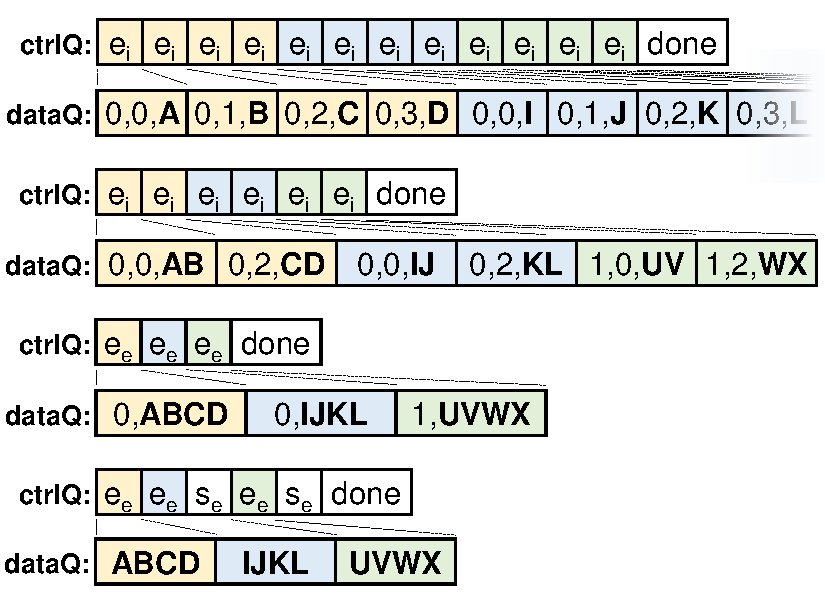
\includegraphics[width=\linewidth, trim={0 3in 0 0},clip]{img_queue_optimizations_impact.pdf}
        \vfill
        \end{minipage}
    \vspace{-0.5em}
    \subcaption{Unoptimized code.}
    \label{fig:ember-dlc-queue-unoptimized-code}
    \end{minipage}
    
    \begin{minipage}{\columnwidth}
        \begin{minipage}{0.45\textwidth}
        \vfill
        \centering
        \begin{lstlisting}[xleftmargin=1em]
while(ctrlQ.pop() == (*$e_i$*)){
  b = dataQ.pop<1 x idx>();
  e = dataQ.pop<1 x idx>();
  v = dataQ.pop<vlen x f32>();
  v_acc(&out[b,e], v);
        \end{lstlisting}
        \vfill
        \end{minipage}
        \begin{minipage}{0.54\textwidth}
        \vfill
        \centering
        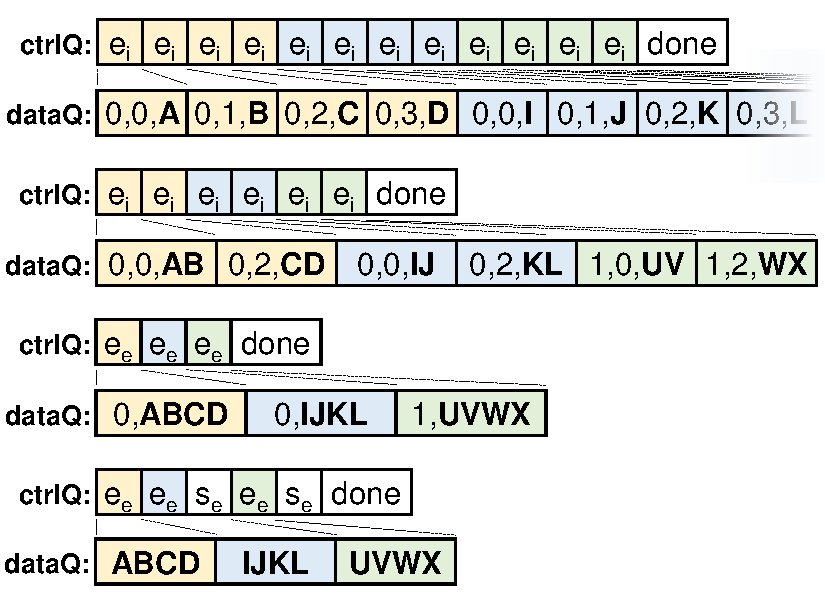
\includegraphics[width=\linewidth, trim={0 2in 0 1in},clip]{img_queue_optimizations_impact.pdf}
        \vfill
        \end{minipage}
    \vspace{-0.5em}
    \subcaption{Vectorized code.}
    \label{fig:ember-dlc-queue-vectorized-code}
    \end{minipage}

    \begin{minipage}{\columnwidth}
        \begin{minipage}{0.45\textwidth}
        \vfill
        \centering
        \begin{lstlisting}[xleftmargin=1em]
while(ctrlQ.pop() == (*$e_e$*)){
  b = dataQ.pop<1 x idx>()
  for(e=0; e<emb_len; e+=vlen){
    v = dataQ.pop<vlen x f32>()
    v_acc(&out[b,e],v) }
        \end{lstlisting}
        \vfill
        \end{minipage}
        \begin{minipage}{0.54\textwidth}
        \vfill
        \centering
        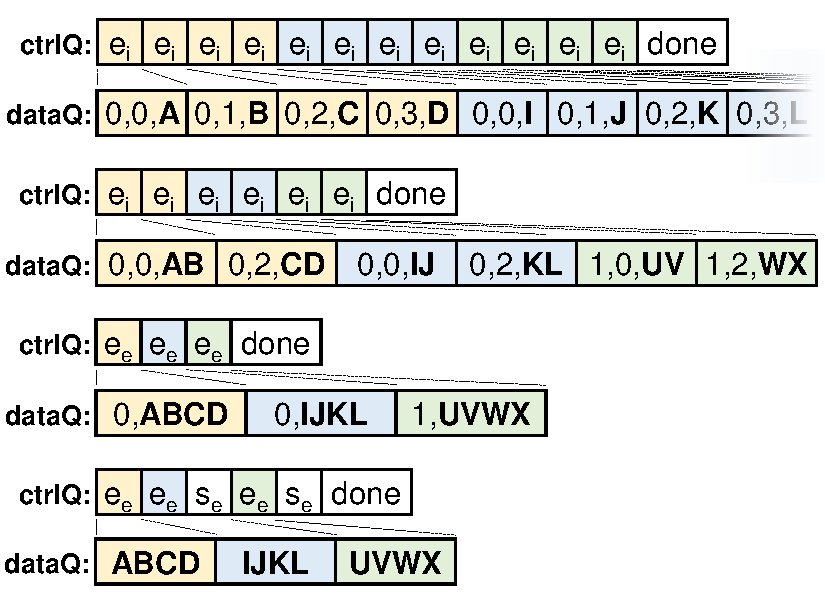
\includegraphics[width=\linewidth, trim={0 1in 0 2in},clip]{img_queue_optimizations_impact.pdf}
        \vfill
        \end{minipage}
    \vspace{-0.5em}
    \subcaption{Buffered code.}
    \label{fig:ember-dlc-queue-buffered-code}
    \end{minipage}

    \begin{minipage}{\columnwidth}
        \begin{minipage}{0.45\textwidth}
        \vfill
        \centering
        \begin{lstlisting}[xleftmargin=1em]
out_ptr = out
while(tkn = ctrlQ.pop() != done){
  if(tkn == (*$e_e$*)){
    for(e=0; e<emb_len; e+=vlen){
      v = dataQ.pop<vlen x f32>()
      v_acc(out_ptr+e, v) }}
  else if(tkn == (*$s_e$*)){
    out_ptr += emb_len }
        \end{lstlisting}
        \vfill
        \end{minipage}
        \begin{minipage}{0.54\textwidth}
        \vfill
        \centering
        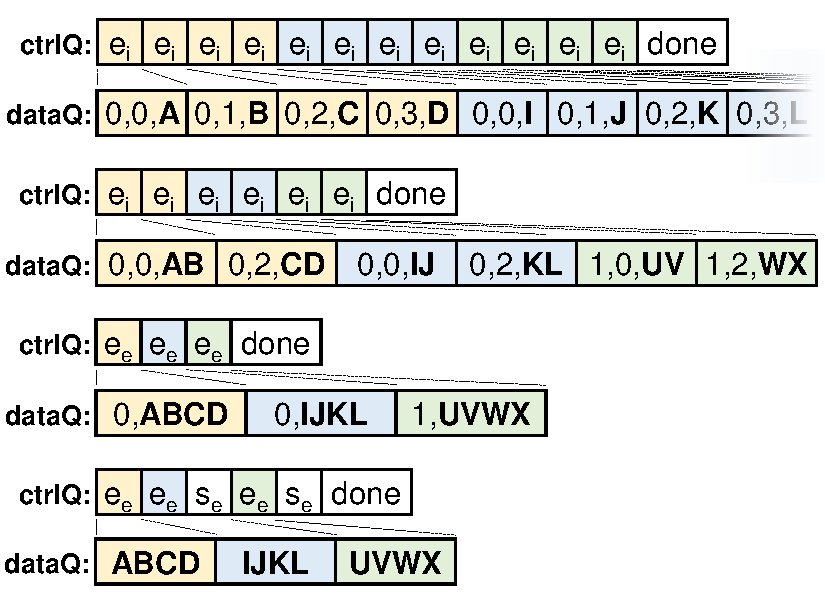
\includegraphics[width=\linewidth, trim={0 0 0 3in},clip]{img_queue_optimizations_impact.pdf}
        \vfill
        \end{minipage}
    \vspace{-0.5em}
    \subcaption{Queue aligned code.}
    \label{fig:ember-dlc-queue-aligned-code}
    \end{minipage}
    
    \caption[Impact of SLC optimizations on DLC queues and compute code.]{Impact of SLC optimizations on DLC EB compute code and output queues. Vectorization widens queued values, buffering groups an entire embedding vector behind one token, and queue alignment removes scalar operands that would otherwise misalign vector data in the queue. Overall, these optimizations reduce queue traffic and improve execute-side vector efficiency.}
    \label{fig:ember-dlc-queue-optimization-impact}
\end{figure}


\begin{figure}
    \centering
    \begin{minipage}{\columnwidth}
    \begin{lstlisting}[basicstyle=\ttfamily\footnotesize]
void eb(idxs: mref<? x idx>, offs: mref<? x idx>,
         vals: mref<? x f32>, out: mref<? x ? x f32>){
  slc.for(str s_b from 0 to num_batches){
    str s_beg = slc.mem_str(offs[s_b]);
    str s_end = slc.mem_str(offs[s_b+1]);
    slc.for(str s_ptr from s_beg to s_end){
      str s_idx = slc.mem_str(idxs[s_ptr]);
      slc.for(str s_e from 0 to emb_len){
        str s_val = slc.mem_str(vals[s_idx,s_e]);
        slc.callback{
          idx b = slc.to_val(s_b);
          idx e = slc.to_val(s_e);
          f32 val = slc.to_val(s_val);
          f32 acc = out[b,e];
          out[b,e] = acc + val; }}}}}
    \end{lstlisting}
    \vspace{-1em}
    \subcaption{Unoptimized code.}
    \label{fig:opt-none}
    \end{minipage}

    \begin{minipage}{\columnwidth}
    \begin{lstlisting}[basicstyle=\ttfamily\footnotesize,firstnumber=7]
      (*\unchanged{str s\_idx = slc.mem\_str(idxs[s\_ptr]); }*)
      slcv.for<vlen>((str s_e, str msk) from 0 to emb_len){
        str s_val = slcv.mem_str<vlen>(vals[s_idx,s_e], msk);
        slcv.callback{
          (*\unchanged{idx b = slc.to\_val(s\_b); }*)
          idx e = slcv.to_val(s_e)[0];
          vec<vlen x f32> val = slcv.to_val<vlen>(s_val);
          vec<vlen x f32> acc = vload<vlen>(out[b,e]);
          vstore<vlen>(acc + val, out[b,e], acc); }}}}}
    \end{lstlisting}
    \vspace{-1em}
    \subcaption{Vectorized code.}
    \label{fig:opt-vec}
    \end{minipage}

    \begin{minipage}{\columnwidth}
    \begin{lstlisting}[basicstyle=\ttfamily\footnotesize,firstnumber=7]
      (*\unchanged{str s\_idx = slc.mem\_str(idxs[s\_ptr]); }*)
      str<vec<vlen x f32>> buf = slcv.buf_str(); // Buffer str
      (*\unchanged{slcv.for<vlen>((str s\_e, str msk) from 0 to emb\_len)\{ }*)
        (*\unchanged{str s\_val = slcv.mem\_str<vlen>(vals[s\_idx,s\_e], msk); }*)
        slc.push(buf, s_val); } // Push into the buffer
      slcv.callback{ // Callback moved at the end of inner loop
        (*\unchanged{idx b = slc.to\_val(s\_b); }*)
        vec<vlen x f32> buf_vec = slc.to_val(buf); // Get buffer
        for(idx e = 0; e < emb_len; e++){ // Iterate buffer
          vec<vlen x f32> val = buf_vec[e]; // Get buffered element
          (*\unchanged{vec<vlen x f32> acc = vload<vlen>(out[b,e]); }*)
          (*\unchanged{vstore<vlen>(acc + val, out[b,e], acc); \}\}\}\}\}\} }*)
    \end{lstlisting}
    \vspace{-1em}
    \subcaption{Buffered code.}
    \label{fig:opt-buf}
    \end{minipage}

    \begin{minipage}{\columnwidth}
    \begin{lstlisting}[basicstyle=\ttfamily\footnotesize,firstnumber=7]
      (*\unchanged{str s\_idx = slc.mem\_str(idxs[s\_ptr]); }*)
      (*\unchanged{str<vec<vlen x f32>> buf = slcv.buf\_str(); }*)
      slcv.for<vlen>((str s_e, str msk) from 0 to emb_len)(idx i=0){
        (*\unchanged{str s\_val = slcv.mem\_str<vlen>(vals[s\_idx,s\_e], msk); }*)
        (*\unchanged{slc.push(buf, s\_val); \} }*)
      (*\unchanged{slcv.callback\{ }*)
        (*\unchanged{vec<vlen x f32> buf\_vec = slc.to\_val(buf); }*)
        (*\unchanged{for(idx e = 0; e < emb\_len; e++)\{ }*)
          (*\unchanged{vec<vlen x f32> val = buf\_vec[e]; }*)
          vec<vlen x f32> acc = vload<vlen>(out[i,e]);
          vstore<vlen>(acc + val, out[i,e], acc); }}}}
    slc.callback{ i++; }}} // end of indices in segment loop
    \end{lstlisting}
    \vspace{-1em}
    \subcaption{Queue aligned code.}
    \label{fig:opt-idx}
    \end{minipage}
    
    \vspace{-0.8em}
    \caption[Progressive DAE optimization steps.]{Progressive optimization of the EB SLC IR. Gray means unchanged.}
    \label{fig:opt-transformations}
\end{figure}

This section first describes three key DAE optimizations enabled by the SLC IR. \Cref{fig:opt-impact,fig:opt-transformations} show how these optimizations transform the SLC IR, compute code, and queues. We also discuss model-specific optimizations and Ember--TMU HW--SW co-design. The common theme is that these optimizations require visibility across the access/execute boundary before queue serialization has been fixed, which is precisely the information preserved by SLC.

%%%%%%%%%%%%%%%%%%%%%%%%%%%%%%%%%%%%%%%%%%%%%%%%%%%%%%%%%%%%%%%%%%%%%%%%%%%%%%%%%%%%%%%%%%%%%%%%%%%%%%%%%%%%%%%%%%%%%%%%%%%%%%%%%%%
\subsubsection{Vectorization} \label{sec:vectorization-ember} %%%%%%%%%%%%%%%%%%%%%%%%%%%%%%%%%%%%%%%%%%%%%%%%%%%%%%%%%%%%%%%%%%%%%%%%%%%%%%
%%%%%%%%%%%%%%%%%%%%%%%%%%%%%%%%%%%%%%%%%%%%%%%%%%%%%%%%%%%%%%%%%%%%%%%%%%%%%%%%%%%%%%%%%%%%%%%%%%%%%%%%%%%%%%%%%%%%%%%%%%%%%%%%%%%

Vectorization is one of the most impactful DAE optimizations (\Cref{sec:dae-potential-scientific,sec:dae-potential-machine-learning}). As shown in \Cref{fig:opt-impact-vec}, for each token, vectorization pops a vector of \textit{vector length (vlen)} elements, improving marshaling and compute efficiency. While auto-vectorizing general code is challenging~\cite{comp2001pub}, the SLC IR provides an effective representation to vectorize loading, marshaling, and computing of embedding operations.

As shown in \Cref{fig:opt-vec}, Ember vectorizes code by converting SLC operations into their vectorized SLCV duals. Unlike the SLC for-loop, the SLCV for-loop (1) adds a \emph{vector length} attribute, (2) instantiates vectorized induction variables, and (3) introduces the concept of \texttt{mask} to handle loop boundaries that are not multiples of the vector length. Masks are used by SLCV streams to perform vectorized index computation and data loading.

We define a \emph{vectorization scheme} as the set of for-loops within a parent loop $p$ and the inner loop $i$, with $p \geq i$, that we intend to vectorize. A for-loop can be vectorized if and only if all of its callbacks can be vectorized. A vectorization scheme is \emph{legal} if and only if all of its for-loops can be vectorized.

Vector extensions such as Arm SVE~\cite{sve2017micro} provide instructions to vectorize most callbacks in embedding operations, making the space of legal vectorization schemes large. However, \Cref{sec:dae-potential-scientific} demonstrates that the most efficient vectorization scheme for sparse-dense tensor multiplication is inner-loop vectorization, assuming the dense tensor is in row-major order and has rows that are larger than the vector length. Embedding operations generally satisfy these assumptions. Hence, like the MLIR sparsifier~\cite{mlirsparse2022taco}, Ember only attempts inner-loop vectorization.

If the inner for-loop is legal, Ember first vectorizes its access code, then its execute code. As a first step, Ember vectorizes the inner for-loop and its streams. As the stream-to-value operations in the callbacks expect stream types, the algorithm adds a temporary cast operation for source materialization. Then, during callback vectorization, Ember recursively vectorizes the uses of these cast operations, producing full SLCV code. %To keep the conversion step simple, load and store operations into callbacks are firstly converted to vector gather and scatter operations, with vector indices and masks coming from its parent vectorized for-loop operation. A further transformation pass simplifies these operations into contiguous vector loads and stores. 

We decided to implement our custom vectorization pass on SLC code rather than vectorizing in SCF before lowering because scalar SCF code is simpler to decouple than vector SCF code that contains complex instructions like mask manipulation, which hinder code analysis. Moreover, SLC exposes both the producing streams and the consuming callbacks, allowing Ember to choose how vector operands should be marshaled through the queue. For instance, an access unit like the TMU can handle out-of-bounds loads in two ways, where the benefit depends on context. The first option sends a mask to the CPU along with the vector operand to indicate the valid vector elements. Although the mask can be directly fed into Arm SVE instructions~\cite{sve2017micro}, mask overhead might impact the performance of tight loops. As a second option, the TMU can send zero-padded vector operands, which is the best choice when embedding vectors are multiples of the architectural vector length.

%%%%%%%%%%%%%%%%%%%%%%%%%%%%%%%%%%%%%%%%%%%%%%%%%%%%%%%%%%%%%%%%%%%%%%%%%%%%%%%%%%%%%%%%%%%%%%%%%%%%%%%%%%%%%%%%%%%%%%%%%%%%%%%%%%%
\subsubsection{Embedding Buffering} \label{sec:bufferization-ember} %%%%%%%%%%%%%%%%%%%%%%%%%%%%%%%%%%%%%%%%%%%%%%%%%%%%%%%%%%%%%%%%%%%%%%%%
%%%%%%%%%%%%%%%%%%%%%%%%%%%%%%%%%%%%%%%%%%%%%%%%%%%%%%%%%%%%%%%%%%%%%%%%%%%%%%%%%%%%%%%%%%%%%%%%%%%%%%%%%%%%%%%%%%%%%%%%%%%%%%%%%%%

The vectorized code in \Cref{fig:opt-impact-vec}, in addition to (de)serializing vector operands, also needs to (de)serialize their positions within the embedding vector (variable \texttt{e}). However, since the size of the embedding vector is fixed, we can generate these positions in the compute unit to reduce queue utilization.

Ember implements this optimization by (de)serializing embedding vectors as compound types. As shown in \Cref{fig:opt-impact-buf}, the access unit pushes into the control queue one $e_e$ (embedding-vector end) token for each embedding vector and, in the data queue, the position of the output embedding vector and all of its values. As the length of the embedding vector (\texttt{emb\_len}) is constant, once the core reads an $e_e$ token, it pops \texttt{emb\_len} elements with a vectorized for-loop. This optimization greatly improves marshaling and compute efficiency.

The SLC IR greatly simplifies this optimization. With the SLC IR, Ember identifies optimization opportunities by examining iteration callbacks for stream-to-value operations whose input is an SLC(V) loop with constant bounds. Then, as shown in \Cref{fig:opt-buf}, Ember initializes a \emph{buffer} stream of vector type (line 8) before the inner SLCV for-loop, where that loop can push the loaded embedding elements (line 11). Finally, Ember moves the inner-loop body callback (lines 10--15 in \Cref{fig:opt-vec}) immediately after the loop (lines 12--18 in \Cref{fig:opt-buf}), adds a stream-to-value operation for the buffer (line 14 in \Cref{fig:opt-buf}), and adds a loop to iterate through it (lines 15--18 in \Cref{fig:opt-buf}). This transformation needs SLC because Ember must still see the loop bounds, the stream that produces each embedding value, and the callback that consumes those values.

Implementing the same optimization in the DLC IR would require complex analyses to reconstruct the dependency chain across the queue that Ember needs to search for optimization opportunities. Implementing the same optimization in the SCF IR is complex since the code is not in DAE form, and Ember would need to integrate such optimization in the decoupling logic, substantially complicating the compiler design. Moreover, since the SCF IR cannot represent DAE code, it would need to lower directly to the DLC IR.

%%%%%%%%%%%%%%%%%%%%%%%%%%%%%%%%%%%%%%%%%%%%%%%%%%%%%%%%%%%%%%%%%%%%%%%%%%%%%%%%%%%%%%%%%%%%%%%%%%%%%%%%%%%%%%%%%%%%%%%%%%%%%%%%%%%
\subsubsection{Queue Alignment} \label{sec:queue-alignment-ember} %%%%%%%%%%%%%%%%%%%%%%%%%%%%%%%%%%%%%%%%%%%%%%%%%%%%%%%%%%%%%%%%%%%%%%%%%%%%%%
%%%%%%%%%%%%%%%%%%%%%%%%%%%%%%%%%%%%%%%%%%%%%%%%%%%%%%%%%%%%%%%%%%%%%%%%%%%%%%%%%%%%%%%%%%%%%%%%%%%%%%%%%%%%%%%%%%%%%%%%%%%%%%%%%%%

Vector loads are more efficient when aligned to cache lines~\cite{eichenberger2004alignment,fireman2007alignment}. However, as shown in \Cref{fig:opt-impact-buf}, the access unit pushes both scalar and vector operands into the data queue. Hence, the vector loads that the execute unit performs from the queue are misaligned by scalar operands. Ember implements two optimizations to align queue accesses according to code characteristics.

For simpler functions like the EB in \Cref{fig:opt-buf}, where all segment IDs are just loop induction variables, Ember stores a reference of these indices in the core and increments them after the loop. This increment is triggered by a segment-end token, $s_e$ in \Cref{fig:opt-impact-idx}.

As shown in \Cref{fig:opt-idx}, Ember implements this optimization by examining iteration callbacks for stream-to-value operations that only read the induction variable of their own SLC(V) loop (e.g. line 13 in \Cref{fig:opt-buf}). Then Ember adds a new variable in the SLC loop (\texttt{i}~variable in line 9 in \Cref{fig:opt-idx}), replaces all uses of the stream-to-value operations with that variable (line 16--17 in \Cref{fig:opt-idx}), and increments it in the end callback of its child loop (line 18 in \Cref{fig:opt-idx}).

However, for more complex models like MP, certain scalars, such as rescaling values, cannot be simplified. In this case, Ember preserves alignment by padding scalars to vectors while generating the DLC IR. As a further optimization, instead of sending segment IDs, Ember offloads full index calculation of partial and output results to the access unit and directly sends addresses to the core, reducing pressure on the core's ALUs.

Similar to embedding buffering, implementing queue alignment in SCF is not possible, and implementing it in the DLC IR requires complex analyses to reconstruct the data flow, control flow, and queue (de)serialization of the input program. Queue alignment requires control flow information to understand where to add the increment callback. It also requires queue (de)serialization to understand which alignment strategy to select. SLC provides both views at once: it exposes which values will cross the queue while preserving the loop structure needed to move or regenerate those values safely.
% Hence, the SLC IR plays a critical role in DAE optimizations.

%%%%%%%%%%%%%%%%%%%%%%%%%%%%%%%%%%%%%%%%%%%%%%%%%%%%%%%%%%%%%%%%%%%%%%%%%%%%%%%%%%%%%%%%%%%%%%%%%%%%%%%%%%%%%%%%%%%%%%%%%%%%%%%%%%%
\subsubsection{Model-Specific Optimizations and HW--SW Co-Design} \label{sec:model-specific-optimizations} %%%%%%%%%%%%%%%%%%%%%%%%%%%
%%%%%%%%%%%%%%%%%%%%%%%%%%%%%%%%%%%%%%%%%%%%%%%%%%%%%%%%%%%%%%%%%%%%%%%%%%%%%%%%%%%%%%%%%%%%%%%%%%%%%%%%%%%%%%%%%%%%%%%%%%%%%%%%%%%

While the optimizations we have presented so far target general embedding operations, we also extended Ember to automatically implement model-specific optimizations. These extensions all follow the same pattern: when a model or format exposes additional structure, Ember represents that structure in SLC/DLC and uses it to specialize the access unit, the queue protocol, or the callback placement. This demonstrates the generality of the SLC IR and our compilation framework, as well as how Ember lends itself to HW--SW co-design.

%%%%%%%%%%%%%%%%%%%%%%%%%%%%%%%%%%%%%%%%%%%%%%%%%%%%%%%%%%%%%%%%%%%%%%%%%%%%%%%%%%%%%%%%%%%%%%%%%%%%%%%%%%%%%%%%%%%%%%%%%%%%%%%%%%%
\paragraph{Cache Utilization} \label{sec:model-specific-optimizations-cache-utilization} %%%%%%%%%%%%%%%%%%%%%%%%%%%%%%%%%%%%%%%%%%%%%%%%%%%%%%%%%%%%%%%%%%%%%%%%%%%%%%%%%%%%%%%%%%%%%%%%%
%%%%%%%%%%%%%%%%%%%%%%%%%%%%%%%%%%%%%%%%%%%%%%%%%%%%%%%%%%%%%%%%%%%%%%%%%%%%%%%%%%%%%%%%%%%%%%%%%%%%%%%%%%%%%%%%%%%%%%%%%%%%%%%%%%%

For instance, block-sparse attention mechanisms exhibit (1)~large structured reuse within each block, (2)~low reuse throughout blocks, and (3)~no computation. Therefore, we extended the SLC IR, DLC IR, and TMU ISA with \emph{store} streams to write directly into memory without passing through the core, and we extended load streams to (1)~select what cache level to read from and (2)~whether to issue (non-)temporal requests. As demonstrated in \Cref{sec:impact-of-model-specific-optimizations}, this greatly improves core and cache utilization. Since the SLC IR preserves code structure, Ember can automatically identify callbacks with no computation, move the store operations into the access unit, and simplify the callback.

%%%%%%%%%%%%%%%%%%%%%%%%%%%%%%%%%%%%%%%%%%%%%%%%%%%%%%%%%%%%%%%%%%%%%%%%%%%%%%%%%%%%%%%%%%%%%%%%%%%%%%%%%%%%%%%%%%%%%%%%%%%%%%%%%%%
\paragraph{Efficient Compression Formats} %%%%%%%%%%%%%%%%%%%%%%%%%%%%%%%%%%%%%%%%%%%%%%%%%%%%%%%%%%%%%%%%%%%%%%%%%%%%%%%%%%%%%
%%%%%%%%%%%%%%%%%%%%%%%%%%%%%%%%%%%%%%%%%%%%%%%%%%%%%%%%%%%%%%%%%%%%%%%%%%%%%%%%%%%%%%%%%%%%%%%%%%%%%%%%%%%%%%%%%%%%%%%%%%%%%%%%%%%

As shown in \Cref{fig:sls-abstraction}, the EB function encodes all indices of all segments in a single vector, while storing the begin and end pointers of each segment in a second vector. This representation closely resembles the CSR (Compressed Sparse Row) format used in sparse linear algebra. However, modern EB implementations~\cite{pytorch2019neurips} typically avoid storing explicit begin and end pointers; instead, they store only the segment lengths and compute boundaries via prefix accumulation. To support this more efficient representation, we extend both the SLC IR and DLC IR with \emph{accumulation streams}, which track EB segment boundaries by accumulating lengths rather than relying on explicit offsets~\cite{dlrm2022mudigere}. This reduces memory overhead and matches contemporary runtime practices.

%%%%%%%%%%%%%%%%%%%%%%%%%%%%%%%%%%%%%%%%%%%%%%%%%%%%%%%%%%%%%%%%%%%%%%%%%%%%%%%%%%%%%%%%%%%%%%%%%%%%%%%%%%%%%%%%%%%%%%%%%%%%%%%%%%%
\paragraph{General Compression Formats} %%%%%%%%%%%%%%%%%%%%%%%%%%%%%%%%%%%%%%%%%%%%%%%%%%%%%%%%%%%%%%%%%%%%%%%%%%%%%%%%%%%%%%%
%%%%%%%%%%%%%%%%%%%%%%%%%%%%%%%%%%%%%%%%%%%%%%%%%%%%%%%%%%%%%%%%%%%%%%%%%%%%%%%%%%%%%%%%%%%%%%%%%%%%%%%%%%%%%%%%%%%%%%%%%%%%%%%%%%%

Another extension targets COO-like formats, which differ fundamentally from CSR-style encodings. In these cases, callbacks cannot be naturally triggered at fiber boundaries, since segment structure is not encoded explicitly. To address this, we introduce \emph{toggle callbacks}, a mechanism that enables computation to be triggered directly on sparse coordinate formats~\cite{phipps2019genten}. This enhancement broadens the applicability of the IR to workloads that rely on COO representations and ensures that compiler-driven optimizations remain effective across diverse sparse tensor formats.


%%%%%%%%%%%%%%%%%%%%%%%%%%%%%%%%%%%%%%%%%%%%%%%%%%%%%%%%%%%%%%%%%%%%%%%%%%%%%%%%%%%%%%%%%%%%%%%%%%%%%%%%%%%%%%%%%%%%%%%%%%%%%%%%%%%
\section{Ember Evaluation} \label{sec:ember-evaluation}
%%%%%%%%%%%%%%%%%%%%%%%%%%%%%%%%%%%%%%%%%%%%%%%%%%%%%%%%%%%%%%%%%%%%%%%%%%%%%%%%%%%%%%%%%%%%%%%%%%%%%%%%%%%%%%%%%%%%%%%%%%%%%%%%%%%

%+++++++++++++++++++++++++++++++++++++++++++++
%++++++++++ START SW CONFIGURATIONS ++++++++++
%+++++++++++++++++++++++++++++++++++++++++++++
\definecolor{Gray}{gray}{0.85}
\begin{table}
  \centering
  %\footnotesize
  \caption[Evaluated code and reference implementations.]{Evaluated code and reference implementations. Ember's evaluated input is structured MLIR generated from sparse machine learning operations; its output is TMU-CPU machine code. In this evaluation, PyTorch programs enter Ember through torch-mlir~\cite{torchmlir2026github}.}
  \vspace{-1em}
\[
\begin{tabular}{lll}
\toprule
  \textbf{Name} & \textbf{MLIR dialects} & \textbf{Description} \\
\toprule
  \texttt{\textbf{emb-opt0}} & \texttt{slc}, \texttt{scf} & unoptimized Ember DAE code \\
  \texttt{\textbf{emb-opt1}} & \texttt{slcv}, \texttt{scf}, \texttt{vector} & \texttt{emb-opt0}+vectorization \\
  \texttt{\textbf{emb-opt2}} & \texttt{slcv}, \texttt{scf}, \texttt{vector} & \texttt{emb-opt1}+bufferization \\
  \texttt{\textbf{emb-opt3}} & \texttt{slcv}, \texttt{scf}, \texttt{vector} & \texttt{emb-opt2}+queue alignment \\
  \texttt{\textbf{ref-dae}}  & \texttt{tmu}, \texttt{scf}, \texttt{vector} & hand-optimized TMU-CPU code \\
\bottomrule
\end{tabular}
\]
  \label{tab:software-versions}
\end{table}
%+++++++++++++++++++++++++++++++++++++++++++
%++++++++++ END SW CONFIGURATIONS ++++++++++
%+++++++++++++++++++++++++++++++++++++++++++

This section demonstrates how Ember enables the full potential of DAE architectures at scale. The evaluation answers three questions. First, does the SLC IR enable optimizations that substantially improve DAE code? Second, can the same framework express model-specific optimizations beyond standard embedding bags? Third, does automatically generated Ember code match handwritten code optimized for our target TMU--CPU system? To answer these questions, we first perform an ablation study on the general embedding optimizations (vectorization, bufferization, and queue alignment) introduced in \Cref{sec:ember-global-optimizations}. We then measure the impact of the model-specific optimizations for LLMs introduced in \Cref{sec:model-specific-optimizations}. Finally, we compare Ember-generated code against hand-optimized implementations.

%%%%%%%%%%%%%%%%%%%%%%%%%%%%%%%%%%%%%%%%%%%%%%%%%%%%%%%%%%%%%%%%%%%%%%%%%%%%%%%%%%%%%%%%%%%%%%%%%%%%%%%%%%%%%%%%%%%%%%%%%%%%%%%%%%%
\subsection{Experimental Methodology} %%%%%%%%%%%%%%%%%%%%%%%%%%%%%%%%%%%%%%%%%%%%%%%%%%%%%%%%%%%%%%%%%%%%
%%%%%%%%%%%%%%%%%%%%%%%%%%%%%%%%%%%%%%%%%%%%%%%%%%%%%%%%%%%%%%%%%%%%%%%%%%%%%%%%%%%%%%%%%%%%%%%%%%%%%%%%%%%%%%%%%%%%%%%%%%%%%%%%%%%

To the best of our knowledge, this is the first work that explores DAE optimizations for embedding operations. As such, the handwritten code we compare Ember against is SCF+VEC MLIR code that we manually decoupled and iteratively optimized through performance analyses with gem5. The experimental setting in this section follows the DAE study in \Cref{sec:dae-potential-machine-learning}. \Cref{tab:software-versions} summarizes the code used in the experiments. This evaluation focuses on the TMU because, among the DAE designs considered in this thesis, it exposes both vectorization and multiple callbacks. We believe similar considerations apply to the other DAE designs the DLC IR can abstract~\cite{spzip2021isca,maple2022isca,planar2021acm}.

%%%%%%%%%%%%%%%%%%%%%%%%%%%%%%%%%%%%%%%%%%%%%%%%%%%%%%%%%%%%%%%%%%%%%%%%%%%%%%%%%%%%%%%%%%%%%%%%%%%%%%%%%%%%%%%%%%%%%%%%%%%%%%%%%%%
\subsection{Impact of General Optimizations} \label{sec:impact-of-general-optimizations} %%%%%%%%%%%%%%%%%%%%%%%%%%%%%%%%%%%%%%%%%%%%%%%%%%%%%%%%%%%%%%%%%%%%
%%%%%%%%%%%%%%%%%%%%%%%%%%%%%%%%%%%%%%%%%%%%%%%%%%%%%%%%%%%%%%%%%%%%%%%%%%%%%%%%%%%%%%%%%%%%%%%%%%%%%%%%%%%%%%%%%%%%%%%%%%%%%%%%%%%

%++++++++++++++++++++++++++++++++++++++++++
%++++++++++ START OPT BREAKDOWN +++++++++++
%++++++++++++++++++++++++++++++++++++++++++
\begin{figure}
\centering
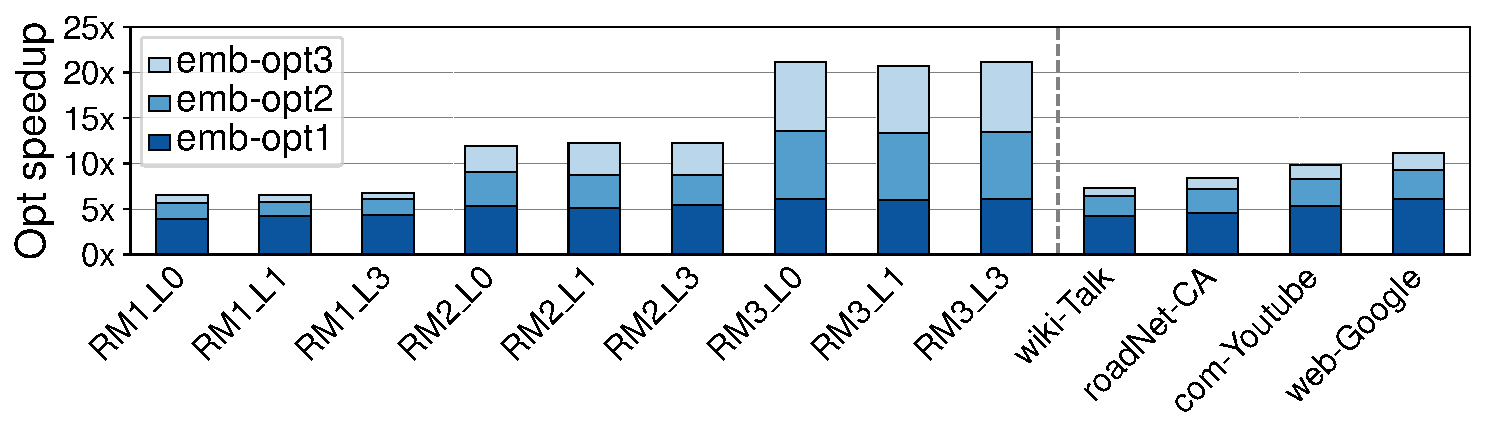
\includegraphics[width=.9\linewidth]{img_opt_speedups.pdf}
\vspace{-1em}
\caption[Performance speedup of Ember optimizations.]{Performance speedup of Ember optimizations on MP models and EB function for various DLRM models (\Cref{tab:dlrm-configurations}) and input locality. All optimizations combined (\texttt{emb-opt3}) improve performance by 6.6$\times$--21$\times$.}
\label{fig:ablation}
\end{figure}
%++++++++++++++++++++++++++++++++++++++++++
%++++++++++ END OPT BREAKDOWN +++++++++++++
%++++++++++++++++++++++++++++++++++++++++++

%++++++++++++++++++++++++++++++++++++++++++
%++++++++++ START OUTQ THROUGHPUT +++++++++
%++++++++++++++++++++++++++++++++++++++++++
\begin{figure}
\centering
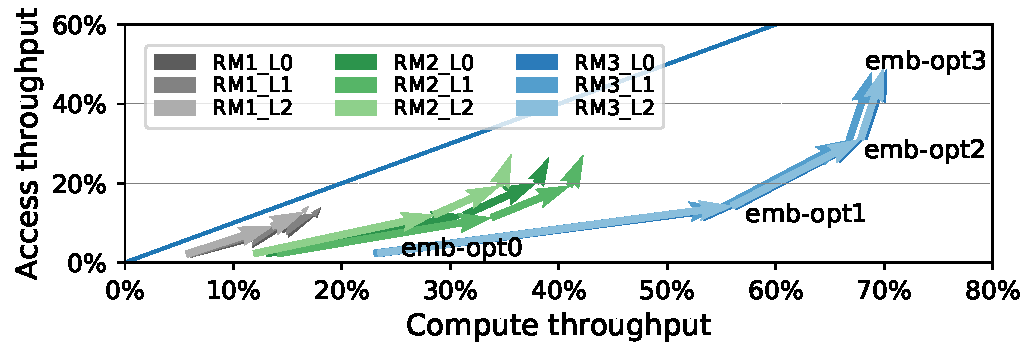
\includegraphics[width=.8\linewidth]{img_rw_optimization_impact.pdf}
\vspace{-0.5em}
\caption[Impact of Ember optimizations on access and compute throughput.]{Impact of Ember optimizations on access throughput (TMU) and compute throughput (CPU). By optimizing both, Ember achieves the highest performance (top-right). }
\label{fig:outq-throughput-improvement}
\end{figure}
%++++++++++++++++++++++++++++++++++++++++++
%++++++++++ END OUTQ THROUGHPUT +++++++++++
%++++++++++++++++++++++++++++++++++++++++++

\Cref{fig:ablation} shows the performance impact of general optimizations such as vectorization (\texttt{emb-opt1}), bufferization (\texttt{emb-opt2}), and queue alignment (\texttt{emb-opt3}) over unoptimized Ember-generated code (\texttt{emb-opt0}) for the EB function and more compute-intensive MP models.

For the EB function, we evaluated the three DLRMs in \Cref{tab:dlrm-configurations}, each running representative synthetic inputs~\cite{dlrm2020hpca} with low (\texttt{L0}), medium (\texttt{L1}), and high (\texttt{L2}) locality. Overall, all optimizations combined (\texttt{emb-opt3}) achieve 6.6$\times$, 12.1$\times$, and 21$\times$ better performance over unoptimized code (\texttt{emb-opt0}) for \texttt{RM1}, \texttt{RM2}, and \texttt{RM3}, respectively. Vectorization is consistently the most impactful optimization with a 5.13$\times$ speedup and only 17\% deviation, whereas other optimizations deliver widely different performance improvements.

To better understand these results, \Cref{fig:outq-throughput-improvement} shows how these optimizations impact the throughput at which the compute unit reads and the access unit writes into the L2 queue. Compute optimizations move upward, whereas memory optimizations move rightward. The blue line indicates where compute-unit throughput equals access-unit throughput. Optimizing only compute code cannot move above the blue line, since the access unit would not be able to marshal enough data to process. This would improve throughput only up to 8$\times$ (\texttt{RM3}, \texttt{emb-opt0}) before the access unit becomes the bottleneck (blue line). However, because of the SLC IR, Ember can perform global optimizations on both access and compute code and move both rightward and upward in the plot, improving performance by up to 21$\times$ (\texttt{RM3}, \texttt{emb-opt3}). For \texttt{RM1}, the most control-intensive model (shorter loops), vectorization already saturates throughput, leaving other optimizations little room for improvement. For \texttt{RM2} and \texttt{RM3}, by reducing coordinate overhead, bufferization helps move closer to the blue line. For \texttt{RM3}, the model with the largest loops, queue alignment removes index overhead, pushing performance closer to the limit.

As shown in \Cref{fig:ablation}, MP models have similar trends, and the optimization impact depends on their compute intensity.

%%%%%%%%%%%%%%%%%%%%%%%%%%%%%%%%%%%%%%%%%%%%%%%%%%%%%%%%%%%%%%%%%%%%%%%%%%%%%%%%%%%%%%%%%%%%%%%%%%%%%%%%%%%%%%%%%%%%%%%%%%%%%%%%%%%
\subsection{Impact of Model-Specific Optimizations} \label{sec:impact-of-model-specific-optimizations} %%%%%%%%%%%%%%%%%%%%%%%%%%%%%%%%%%
%%%%%%%%%%%%%%%%%%%%%%%%%%%%%%%%%%%%%%%%%%%%%%%%%%%%%%%%%%%%%%%%%%%%%%%%%%%%%%%%%%%%%%%%%%%%%%%%%%%%%%%%%%%%%%%%%%%%%%%%%%%%%%%%%%%

\begin{figure}
    \centering
    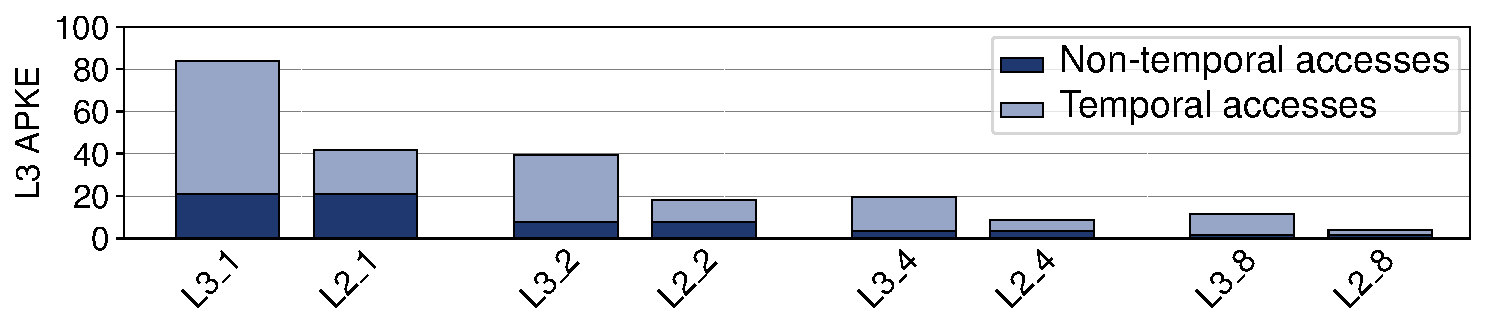
\includegraphics[width=.8\linewidth]{img_llm_opt.pdf}
\caption[Impact of cache optimizations for sparse LLMs.]{L3 Accesses Per Kilo Element (APKE) of the BigBird gather function with different block sizes (1, 2, 4, and 8) and TMU configurations. Temporal accesses load indices and non-temporal accesses load embedding vectors. Reading from L2 substantially helps filter LLC accesses.}
    \label{fig:l3-accesses}
\end{figure}

As discussed in \Cref{sec:model-specific-optimizations}, Ember lends itself to model-specific optimizations. \Cref{fig:l3-accesses} shows that, in block-sparse attention mechanisms, loading highly reused embedding blocks from L2 rather than LLC filters 67\%---74\% of the embedding reads and 50\%---65\% of the overall accesses, which include non-temporal loads for indices, with larger reductions on larger block sizes with more intrinsic reuse. By directly writing data with the store streams instead of going through the core, Ember enables efficient gather operations with low resource utilization.

%%%%%%%%%%%%%%%%%%%%%%%%%%%%%%%%%%%%%%%%%%%%%%%%%%%%%%%%%%%%%%%%%%%%%%%%%%%%%%%%%%%%%%%%%%%%%%%%%%%%%%%%%%%%%%%%%%%%%%%%%%%%%%%%%%%
\subsection{Comparison with Hand-optimized Code} \label{sec:comparison-with-hand-optimized-code} %%%%%%%%%%%%%%%%%%%%%%%%%%%%%%%%%%%%%%%%%%%%%%%
%%%%%%%%%%%%%%%%%%%%%%%%%%%%%%%%%%%%%%%%%%%%%%%%%%%%%%%%%%%%%%%%%%%%%%%%%%%%%%%%%%%%%%%%%%%%%%%%%%%%%%%%%%%%%%%%%%%%%%%%%%%%%%%%%%%

%++++++++++++++++++++++++++++++++++++++++++++
%++++++++++ START EMBER VS HANDOPT ++++++++++
%++++++++++++++++++++++++++++++++++++++++++++
\begin{figure}
\centering
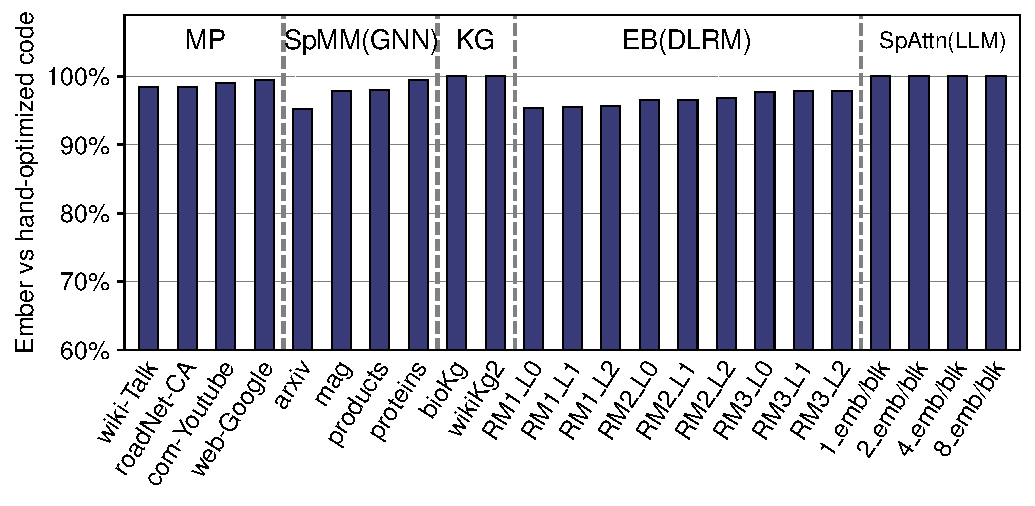
\includegraphics[width=.8\linewidth]{img_ember_vs_handopt.pdf}
\vspace{-0.5em}
\caption[Performance of Ember generated code.]{DAE code automatically generated and optimized by Ember (\texttt{emb-opt3}) achieves a geomean 99\% performance compared to hand-optimized code (\texttt{ref-dae}) across the different model classes in \Cref{sec:characterization-and-implications}.}
\label{fig:ember-vs-handopt}
\end{figure}
%++++++++++++++++++++++++++++++++++++++++++
%++++++++++ END EMBER VS HANDOPT ++++++++++
%++++++++++++++++++++++++++++++++++++++++++

\Cref{fig:ember-vs-handopt} shows the performance of DAE code automatically generated and optimized by Ember (\texttt{emb-opt3}) compared to hand-optimized code (\texttt{ref-dae}) for all model classes in \Cref{sec:characterization-and-implications}. Besides all optimizations discussed in \Cref{sec:ember-global-optimizations}, hand-optimized code also includes low-level, CPU-specific optimizations to improve callback invocations. These CPU-specific optimizations include, for instance, (1)~reordering the if-cases of multi-callback code (e.g. \Cref{fig:opt-impact-idx}) according to their taken frequency or (2)~setting the values of control tokens so they can be directly used in compute code (e.g. to increment variables).

Overall, these CPU-specific optimizations primarily affect multi-callback code such as MP, EB, and SpMM, yielding performance improvements of up to 5\%, with an average geometric mean improvement of 1\%. The limited impact of these low-level optimizations arises because, as discussed in \Cref{sec:impact-of-general-optimizations}, the optimizations introduced in \Cref{sec:ember-global-optimizations} already push the architecture close to its limits, leaving little room for further gains. Nevertheless, because these low-level optimizations are highly CPU-specific, we chose not to integrate them into Ember, which is designed to provide a more general solution for a larger class of architectures.

Ultimately, we believe that the optimizations presented in \Cref{sec:ember-global-optimizations} are sufficient to fully unlock the potential of the DAE architectures and embedding operations studied in this thesis. Ember targets structured sparse--dense and embedding-style loops; it does not attempt to compile arbitrary pointer-heavy programs or general control flow to DAE hardware.

\section{Summary}

This chapter introduced Ember, a compiler stack for generating optimized DAE code from structured sparse machine learning operations. The central challenge is that SCF retains the input program structure but does not expose queue-based decoupling, whereas DLC exposes decoupling but loses the global control-flow and data-flow information needed for optimization. Ember addresses this with the SLC IR, which represents access streams, compute callbacks, and stream-to-value uses in a structured form. This enables vectorization, embedding buffering, queue alignment, and model-specific optimizations before lowering to explicit DLC queues and target-specific TMU--CPU code. The evaluation shows that these optimizations improve generated code by 6.6$\times$--21$\times$ over unoptimized DAE code and achieve 99\% of hand-optimized performance, removing the need for users to manually write DAE programs.
